\documentclass{article}
\usepackage[utf8]{inputenc}

\title{MATH3160 — Portfolio 1.1-2.1}
\author{Mike Medved}
\date{September 4th, 2022}

\usepackage{color}
\usepackage{amsthm}
\usepackage{amssymb} 
\usepackage{amsmath}
\usepackage[margin=1in]{geometry} 
\usepackage{listings}
\usepackage[dvipsnames]{xcolor}
\usepackage{tikz}

\begin{document}

\maketitle

\section{Deliverables}

\subsection{Sample Space}

\textbf{Definition:} The Sample Space S with respect to an Experiment E is a the set of all possible outcomes for the given experiment.

\subsubsection{Examples}

\begin{itemize}
    \item A coin flip has a sample space of $\{H, T\}$.
    \item A die roll has a sample space of $\{1, 2, 3, 4, 5, 6\}$.
\end{itemize}

\break
\subsection{Set Operations}
\begin{itemize}
    \item Set Union:
    $\hfill \break$
    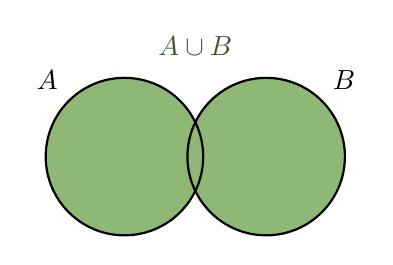
\begin{tikzpicture}[thick,
        set/.style = {circle,
        minimum size = 2cm,
        fill=OliveGreen!50}]]

        % Set A
        \node [set,label={135:$A$}] (A) at (0,0){};
            
        % Set B
        \node [set,label={45:$B$}] (B) at (1.8,0){};
            
        % Circles outline
        \draw (0,0) circle(1cm);
        \draw (1.8,0) circle(1cm);
            
        % Union text label
        \node[OliveGreen!50!black] at (0.9,1.4) {$A\cup B$};
            
    \end{tikzpicture}

    \item Set Intersection:
    $\hfill \break$
    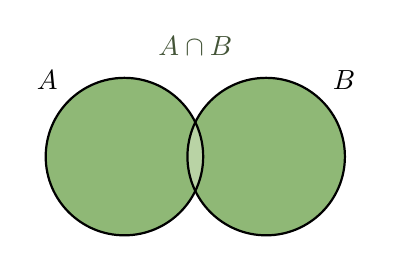
\begin{tikzpicture}[thick,
        set/.style = {circle,
            minimum size = 2cm,
            fill=OliveGreen!50}]
     
        % Set A
        \node[set,label={135:$A$}] (A) at (0,0) {};
        
        % Set B
        \node[set,label={45:$B$}] (B) at (1.8,0) {};
        
        % Intersection
        \begin{scope}
            \clip (0,0) circle(1cm);
            \clip (1.8,0) circle(1cm);
            \fill[OliveGreen!30](0,0) circle(1cm);
        \end{scope}
        
        % Circles outline
        \draw (0,0) circle(1cm);
        \draw (1.8,0) circle(1cm);
        
        % Set intersection label
        \node[OliveGreen!50!black] at (0.9,1.4) {$A\cap B$};
     
    \end{tikzpicture}
 
    \item Set Difference:
    $\hfill \break$
    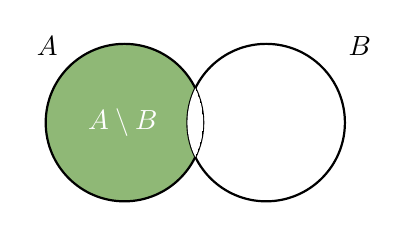
\begin{tikzpicture}[thick,
        set/.style = { circle, minimum size = 2cm}]
     
        % Set A
        \node[set,fill=OliveGreen!50,label={135:$A$}] (A) at (0,0) {};
        
        % Set B
        \node[set,fill=white,label={45:$B$}] (B) at (0:2) {};
        
        % Circles outline
        \draw (0,0) circle(1cm);
        \draw (1.8,0) circle(1cm);
        
        % Intersection
        \begin{scope}
            \clip (0,0) circle(1cm);
            \clip (1.8,0) circle(1cm);
            \fill[White](0,0) circle(1cm);
        \end{scope}

        % Difference text label
        \node[left,white] at (0.55, 0){$A \setminus B$};
     
    \end{tikzpicture}

    \item Symmetric Difference: $A \triangle B$
    $\hfill \break$
    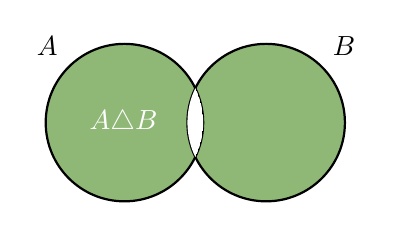
\begin{tikzpicture}[thick,
        set/.style = {circle,
            minimum size = 2cm,
            fill=OliveGreen!50}]
     
        % Set A
        \node[set,label={135:$A$}] (A) at (0,0) {};
        
        % Set B
        \node[set,label={45:$B$}] (B) at (1.8,0) {};
        
        % Circles outline
        \draw (0,0) circle(1cm);
        \draw (1.8,0) circle(1cm);
        
        % Intersection
        \begin{scope}
            \clip (0,0) circle(1cm);
            \clip (1.8,0) circle(1cm);
            \fill[White](0,0) circle(1cm);
        \end{scope}

        % Set intersection label
        \node[left,white] at (0.55, 0){$A \triangle B$};
     
    \end{tikzpicture}

    \item Set Disjoint: $A \bot B$
    $\hfill \break$
    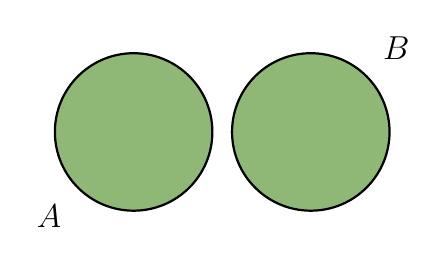
\begin{tikzpicture}[thick,
        set/.style = {circle,
            minimum size = 2cm,
            fill=OliveGreen!50}]
    
        % Circle with label distance 0.5cm
        \node[draw,
            circle,
            minimum size =2cm,
            fill=OliveGreen!50,
            label={[label distance=0.1cm,font=\large]225:$A$}] (circle1) at (0,0){};
        
        % Circle with large label font
        \node[draw,
            circle,
            minimum size =2cm,
            fill=OliveGreen!50,
            label={[label distance=0.1cm,font=\large]45:$B$}] (circle2) at (2.25,0){};
        
    \end{tikzpicture}

    \item Set Inclusion:
    $\hfill \break$
    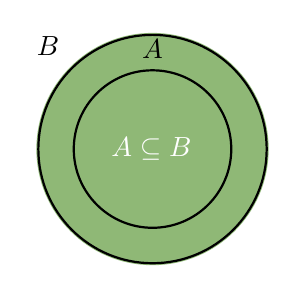
\begin{tikzpicture}[thick,
        set/.style = {circle,
            minimum size = 2cm,
            fill=OliveGreen!50},
        largerSet/.style = {circle,
            minimum size = 2.95cm,
            fill=OliveGreen!50}]
        
        % Set A
        \node[largerSet,label={135:$B$}] (A) at (0,0) {};
        
        % Set B
        \node[set,label={90:$A$}] (B) at (0,0) {};

        % Circles outline
        \draw (0,0) circle(1cm);
        \draw (0,0) circle(1.45cm);

        % Set inclusion label
        \node[left,white] at (0.625, 0){$A \subseteq B$};
    \end{tikzpicture}

    \item Set Compliment:
    $\hfill \break$
    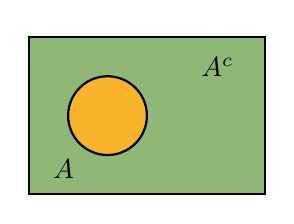
\begin{tikzpicture}[thick,
        set/.style = {circle,
            minimum size = 1cm,
            fill=Dandelion}]

        % Sample Space
        \draw[black,thick,fill=OliveGreen!50] (0,0) rectangle (3,2);
        
        % Set A
        \node[set, label={235:$A$}] (A) at (1,1) {};
        \node[label={295:$A^c$}] (B) at (2,2) {};

        % Circles Outline
        \draw (1,1) circle(0.5cm);
    \end{tikzpicture}
\end{itemize}

\subsection{Events $\Leftrightarrow$ Sets}
\begin{table}[h]
    \begin{tabular}{|l|l|}
    \hline
    \textbf{Event}          & \textbf{Set}                              \\ \hline
    Sure Event              & $\mathbf{S}$ (Entire Sample Space)        \\ \hline
    Impossible Event        & $\emptyset$ (Empty Set)                   \\ \hline
    Event A                 & The subset all of favorable outcomes to A \\ \hline
    Event A or B            & A $\cup$ B                                \\ \hline
    Event A and B           & A $\cap$ B                                \\ \hline
    Event A implies B       & Set B is included in Set A                \\ \hline
    Event A, B incompatible & Set A and Set B are disjoint              \\ \hline
    Contrary of Event A     & $A^c$ with respect to the sample space S  \\ \hline
    \end{tabular}
\end{table}

\subsection{Combinatorics: n-choose-k}

\textbf{Definition:} The number of ways of choosing $k$ objects from a set of $n$ objects is denoted by $\binom{n}{k}$.

$\hfill \break$
This can be accomplished by utilizing the following formula, where $n$ represents the number of elements in the set, and $k$ represents the amount being chosen.

$$
\binom{n}{k} = \frac{n!}{k!(n-k)!}
$$

\subsubsection{Examples}
\begin{itemize}
    \item Given the set $N = \{1, 2, 3, 4, 5, 6, 7\}$, how many ways are there to choose 3 \textit{ordered} objects from N?
    \begin{itemize}
        \item For the first entry, there are seven possibilities, for the second entry, there are six possibilities, and so on. Therefore, according to the definition of \textbf{n-choose-k}, there are $7*6*5$ different choices for choosing three ordered elements from the seven element set.
    \end{itemize}
    \item Given the same set $N$, how many ways are there to choose 3 \textit{different} objects from N?
    \begin{itemize}
        \item There are $\frac{7!}{4!*3!}$ ways to choose three different objects from the set.
    \end{itemize}
\end{itemize}

\subsection{Binomial Theorem}

\subsection{Classical Definition of Probability}

\subsection{Axiomatic Definition of Probability}

\end{document}